\section{Analyse}
  \subsection{Définition du sujet}
    
    % Petite intro / Definition dans les très grandes lignes du sujet
    Une problématique récurrente dans le monde informatique est
    l'optimisation des ressources disponibles. Dans un réseau les
    ressources sont souvent inégalement utilisées. Une meilleure
    utilisation de ces ressources pourrait être obtenu en permettant à
    ces machines de s'échanger des tâches. C'est le but d'un système
    de répartition de charge.
        
    Afin de mieux comprendre ce qui est demandé voici quelques
    définitions des termes techniques employés.
    
    \paragraph{Tâche} Dans notre système une tâche l'execution d'un
      programme. On pourra considérer plus tard le degré
      d'interactivité que l'on souhaite gérer (gestion des E/S
      standards, gestion des fichiers, interface graphique...)
      
    %\paragraph{Un n\oe{}ud, un site} Une station de travail UNIX dans
    %  l'implémentation demandé

    \paragraph{Placement réparti} Ordonnancement de programmes i.e. choix
      d'un processeur pour un processus parmis un ensemble de
      machines. C'est une manière de tirer parti des ressources
      inutilisées.
      
    % Dynamique à détailler si on a le temps
    \paragraph{Placement dynamique et statique} Dans le cadre du
      placement statique avant le démarrage du système de répartion sera
      associé à une tâche un processeur. Cette tâche ne pourra
      qu'être executé sur ce processeur même si celui-ci est
      surchargé. Dans le cadre du placement dynamique le processeur où
      s'executera une tâche sera déterminé pendant l'execution.
              
    % TODO bonus - Eventulement accompagner d'un schéma comme celui du cours de Folliot
    \paragraph{Partage et équilibrage de charge} Il existe deux grandes
      stratégies de placement dynamique. La première stratégie est
      nommée partage de charge. Lorsque la charge globale d'une
      machine dépasse un seuil caractérisant la surcharge, il devient
      nécessaire de déplacer quelques unes de ces tâches. Le but du
      partage de charge est de maximiser le débit d'exécution moyen
      des tâches. La seconde stratégie de placement est nommée
      équilibrage de charge. À chaque instant le système de
      répartition essaye de conserver un équilibre dans la répartition
      de la charge globale. Pour cela il determine une charge idéale
      que chacune des machines tend à expérimenter. Cette charge
      idéale est la moyenne des charges individuelles du système.

    %\paragraph{Coopératif} Placement décidé grâce à la coopération
    %  de l'ensemble des machine.

    %\paragraph{Connaissance de l'état global} La coopération permet
    %  d'avoir une réprésentation de l'ensemble du système (cependant
    %  inexacte du au temps de transmissions de données).

    \paragraph{Centralisation} Si l'on considère une implémentation
      décentralisé de ce système alors chaque n\oe{}ud a les mêmes
      prérogatives. Chaqun doit connaitre l'état du système ce qui
      impose soit un échange important de message passant
      difficilement à l'échelle soit un système d'échange
      d'information entre les n\oe{}ud complexe (connaissance
      partielle de l'état du système sur un n\oe{}ud). De plus, cela
      implique une connaissance approximative de l'état du système.
      Une approche centralisé defini les n\oe{}uds comme esclave
      soumis à un n\oe{}ud spécifique coordinateur. Quand un n\oe{}ud
      souhaite transferer une tâche, il envoie une demande au
      coordinateur qui choisit alors un n\oe{}ud cible en utilisant
      l'ensemble des information à sa disposition. On parlera aussi
      d'approche maitre-esclave ou bien client-serveur.      
      
    \paragraph{}
    L'objectif de ce projet est d'aboutir à la mise en \oe{}uvre
    effective d'un ordonnancement de processus sur un ensemble des
    machine. C'est à dire, à un instant donnée, déterminer le
    placement d'une tâche sur la machine la plus capable de la traiter
    en fonction de la charge de chacune des machines du parc. Le
    programme consiste en une couche d'abstraction intermediaire entre
    le système d'exploitation et les programmes à executer.
        
    \begin{figure}[h!]
      \centering
      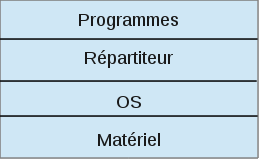
\includegraphics[width=0.58\textwidth]{img/couches_du_systeme.png}
      \caption{Couches d'abstrations présente dans un noeud}
    \end{figure}
    
  % Dans cette partie on doit définir toutes les problématiques associé
  % càd à quelles questions on devra répondre dans la partie conception
  \subsection{Compréhension des problèmes}
    
    La mise en place d'une telle solution pose un ensemble de
    questions auquelles il est nécessaire de répondre. Il est évoqué
    dans le sujet quatres grandes problématiques lié à la répartition.

    \begin{itemize}
      \item Evaluation de la charge de chaque machine
      \item Definition de la surcharge
      \item Choix de la tâche à déplacer 
      \item Choix des machines
    \end{itemize}

    Pour chacune de ces questions il est nécessaire de définir une
    politique définissant la manière dont on y répond. Aux politique
    répondant à ces questions s'ajoute une politique de tolérance aux fautes.

    \subsubsection{Politique d'information}

      Par définition, le système étant réparti il y a une dispersion
      des données importante. Le module d'information consiste à
      définir les informations devant être collectées, les instants
      pendant lesquels ces informations sont collectées, à partir de
      quels n\oe{}uds elles sont collectées.

      % A completer?
      \paragraph{Évaluation de la charge} Une bonne évaluation de la
        charge est cruciale pour notre appliction, l'efficacité et la
        réactivité de notre application en dépend. La charge de chaque
        machine constitue donc une information essentielle devant être
        recueillie. 

      % Mettre un schema?
      \paragraph{Répartition de l'information} Il existe deux méthodes
        de récolte d'information de la charge. La première est une
        politique où l'information est récoltée à la demande, ce qui
        permet de minimiser le nombre de messages échangés. Le
        principal inconvénient étant que l'information peut ne pas
        être suffisamment à jour dans le cas où les évenements qui
        lancent la récolte ne se produisent pas assez souvent. La
        seconde est une politique où l'information est récoltée
        périodiquement. Avec cette méthode la définition de la période
        est cruciale, trop grande on retrouvera le même inconvenient
        qu'avec une récolte évenementielle, trop petite les messages
        de contrôles risquent de saturer le réseau.
      
    \subsubsection{Politique de transfert}

      Le module de transfert est responsable de déterminer si un
      n\oe{}ud est dans un état approprié pour participer à un
      transfert de tâche comme source ou comme receveur.

      \paragraph{Évalutation de la surcharge} Afin de décider s'il est
        possible ou necessaire de faire un transfert il est possible
        de se référer à un seuil au delà du quel on considère être
        surchargé. Ce seuil peut être fixe ou bien dynamique,
        dépendant de l'activité du système de répartition.

      \paragraph{Décision de placement} Dans le cas du partage de
        charge, lors du dépassement de seuil de surcharge il est
        necessaire d'emetter une décision de placement pour chaque
        nouvelle tâche.  Dans le cas de l'équilibrage de charge un
        décision est requise à chaque nouvelle tâche sans contrainte
        de seuil.

    \subsubsection{Politique de localisation}

      Ce module est responsable de trouver les n\oe{}uds, émetteur et
      recepteur, étant les meilleures candidats au transfert d'une
      tâche. On répond donc ici au problème du choix de la machine
      réceptrice.

      \paragraph{Approche serveur} La première approche basée sur
        un modèle serveur consiste à permettre aux machines pouvant
        accueillir des tâches supplémentaires de proposer leurs
        services. Lorsqu'une machine estime pouvoir accueillir une
        tâche elle émet une offre de service. Les n\oe{}uds subissant
        une surcharge répondent en conséquence. La machine détermine
        alors le n\oe{}ud le plus approprié à ce transfert de tâche.

      \paragraph{Approche client} La seconde approche, à l'inverse,
        se base sur le modèle \textit{client} et consiste à permettre
        aux machines subissant une surcharge de demander les services
        d'une des autres machines du système. Lorsqu'une machine
        souhaite transferer une tâche elle emet une demande de partage
        de charge. Les n\oe{}uds aptes à offrir leur aide répondent en
        conséquence. La machine détermine alors le n\oe{}ud le plus
        approprié.
          
     %\paragraph{} Dans la pratique le choix d'un approche dépendra
     %   fortement si l'on est dans un système avec centralisation ou
            
    %\subsubsection{Politique de séléction}
    %  La politique de sélection est responsable du choix des tâches à
    %  transférer. Nous distinguons trois politiques principales de
    %  sélection.

    %  \begin{itemize}
    %    \item choisir une des tâches ayant contribué à ce que le nœud 
    %            devienne surchargé.
    %    \item choisir n'importe quel tâche c'est à dire toute les 
    %            tâches sont considérées comme éligibles.
    %    \item choisir une tâche approprié. Le choix d'une tâche 
    %           appropriée peut nécessiter une bonne connaissance sur la
    %            tâche aussi bien que sur les machines destinataire.
    %  \end{itemize}
        
    % NB on doit gerer une machine qui tombe, mais pas un remise en route auto
    \subsubsection{Politique de tolérance aux fautes}

      On doit gérer les pannes franches des machines, c'est-à-dire les
      machines ne répondant plus. D'une part on doit pouvoir détecter
      la panne ce qui implique d'interoger chaque machine à intervalle
      de temps réguilier. D'autre part, on doit faire en sorte que la
      panne ne pertube pas le bon déroulement de notre système. On
      pourra donc spécifier explicitement que les tâches interrompues
      ne se sont pas terminée correctement. Ainsi, la machine les
      ayant transféré pourra de nouveau les faire executer dans le
      système réparti.

\newpage
\section{Conception}

  Dans cette partie, nous allons nous intéresser aux données présentes
  sur chaque n\oe{}ud, aux messages envoyés entre sites et aux
  algorithmes de chacun des modules étudiés ci-dessus.

  \subsection{Topologie}

    Par soucis de simplicité et de faisabilité -- n'ayant jamais
    implémenté de système réparti -- nous organiserons notre système
    de placement selon un modèle maître-esclaves. En effet, la
    centralisation des données simplifie la réalisation d'un tel
    système. Le rôle d'un esclave est de participer au placement
    réparti nottamment en exécutant les tâches qui lui sont
    confiées. Il a connaissance de l'identité du maître ainsi que de
    sa propre charge. Le rôle du maître est de coordoner le placement
    réparti. Ainsi, le placement est réalisé en centralisant les
    données ainsi que la prise de décision. Le maître a connaissance
    de tous les esclaves ainsi que de la charge de chacun des
    esclaves. La machine maître endosse le double rôle de maître
    et d'esclave.
        
    \begin{figure}[h!]
      \centering
      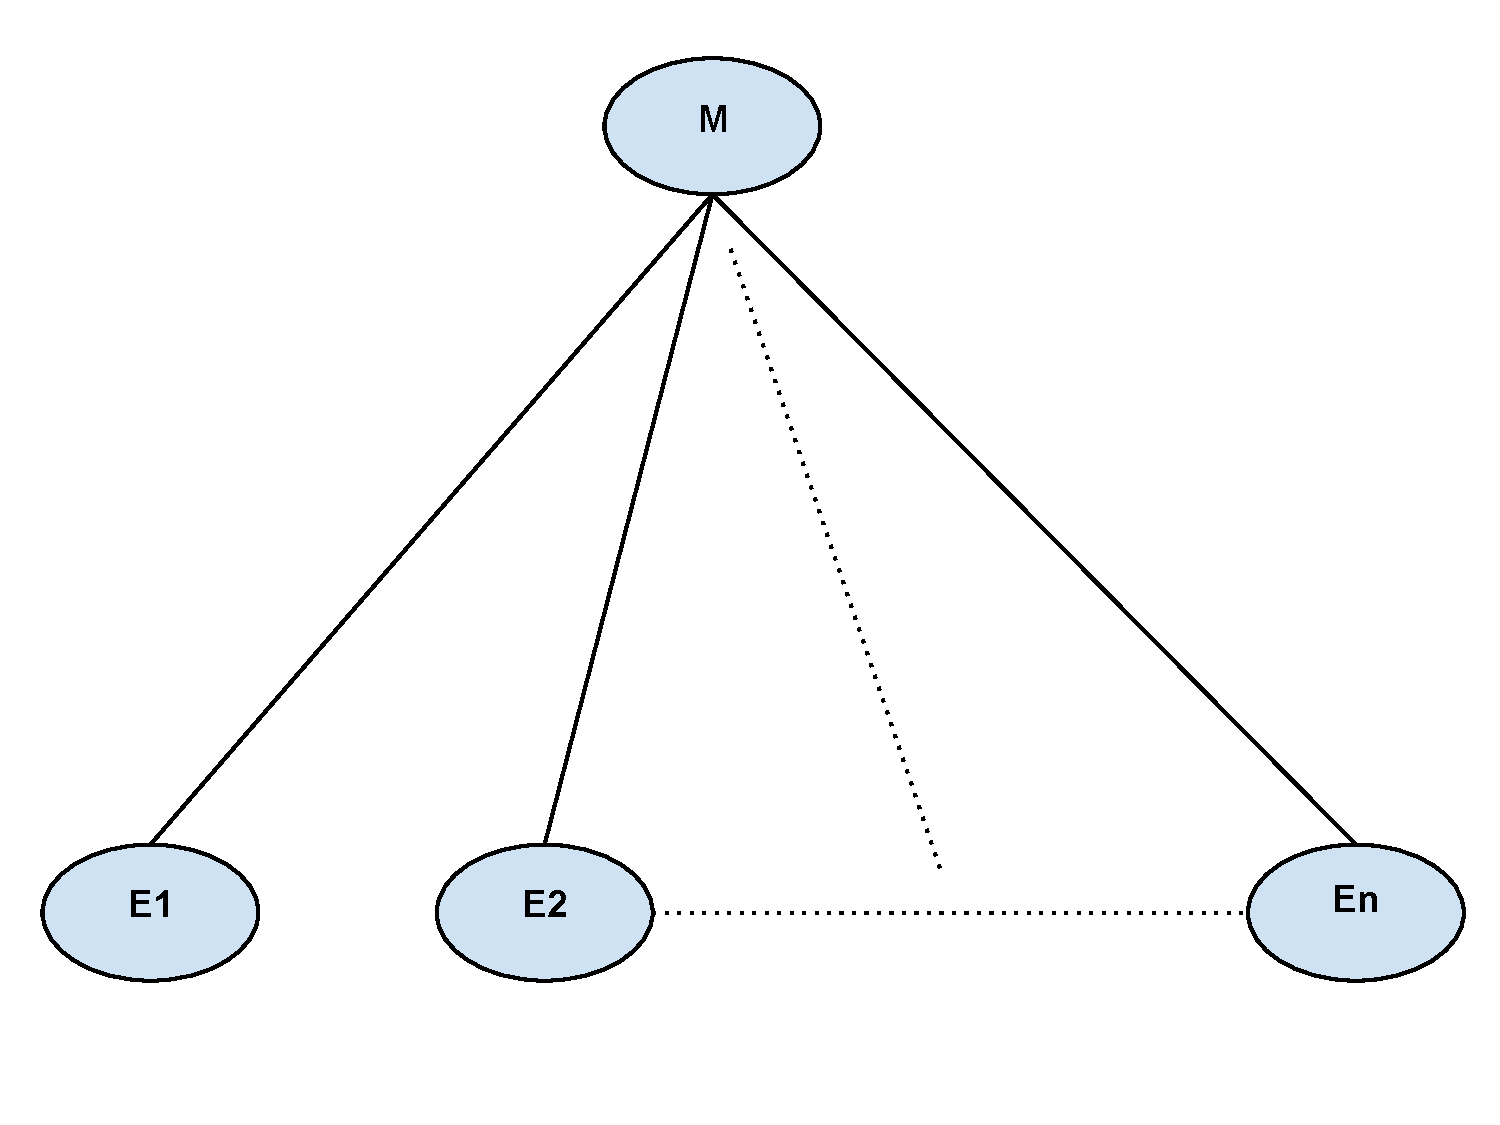
\includegraphics[scale=0.45]{img/topologie.pdf}
      \caption{Topologie du système de placement réparti}
    \end{figure}
      
    % petit argumentation sur les autre possibilité et les raison du
    % choix

    Notons que cette solution peut poser problème dans le cas d'une
    machine maitre peu performante ou d'un nombre d'esclave trop
    grand. Un système totalement décentralisé effacerai le problème de
    goulot d'étrangelement au niveau du maîtere. Compte-tenu des
    exigences de notre projet, on peut imaginer que le nombre de
    machines restera raisonnable (inférieure à 20), ainsi la gestion
    des esclaves par un ordinateur de bureau récent restera trés
    largement supportable.
        
  \subsection{Interface utilisateur}

    Concernant les interaction avec l'utilisateur nous avons choisi la
    voie de la simplicité. L'application se lancera via un terminal.
    A l'interieur de l'application l'interface sera en ligne de
    commande avec un nombre de commandes réduit. Chaque commande
    traitera une opération bien distincte.

    \begin{itemize}
      \item S'integer au système
      \item Executer une tache dans système réparti
      \item Quitter l'application
      \item Observer le système
    \end{itemize}
        
  \subsection{Calcul de la charge d'une machine}

    Il est capital de définir correctement ce que sera la charge dans
    notre application afin d'obtenir de bonnes performances. Une
    solution simple est de considérer le nombre de processus à l'état
    prêt, attendent le processeur. Il faudra considérer l'ensemble des
    processus c'est-à-dire aussi ceux s'executant en dehors du système
    de placement réparti. Afin de renforcer la validité d'utilisation
    de ce facteur on pourra le pondérer en fonction des particularités
    de chaque machine.
      
    \subsection{Module d'information}

      Ce module concerne la gestion de l'état ainsi que de la charge
      du système. Compte-tenu de la topologie choisie, les
      informations gobales seront centralisés au niveau du maître. Il
      devra gérer deux ensembles de données à savoir l'état des
      clients et la charge des client.
        
      Les donnés seront récupéré par interrogation (polling) des
      esclaves par le maître. Chaque esclave recalcule sa charge à
      chaque fois que le maitre lui enverra une requête. Le polling se
      fera dès lors que le système aura besoin de données à jour.

      %\begin{itemize}
      %  \item polling de tout les esclaves lorsque le maître cherche à
      %          placer une nouvelle tâche.
      %  \item polling de tout les esclaves lors de l'élection d'un 
      %          nouveau maître.
      %  \item polling de tout les esclaves lorsque l'utilisateur
      %          demande l'état du système.
      %  \item polling du nouvel arrivant lors de l'insertion d'une
      %          nouvelle machine
      %\end{itemize}

    \subsection{Module de transfert}

      Afin de minimiser les échanges entre les différents sites, on
      laisse la possibilité aux esclaves d'exécuter leurs propres
      tâches sans passer par le maître. le transfert de tâche sera
      uniquement effectué lorsque l'escalve se considérera surchargé.
      Dans ce cas de figure il demandera au maître une machine
      destinatrice sur laquelle il pourra envoyer la tâche.
        
      \paragraph{Cas partage} C'est la politique de placement que nous
        implémenterons dans un premier temps. Chaque esclave possede
        un seuil qui lui est propre. Au départ le seuil sera fixe.
      
      \paragraph{Cas équilibrage} Cette politique sera mise en place
        dans un second temps. Le seuil sera calculé par le maître
        comme une moyenne des charges des esclaves.

    \subsection{Module de localisation}

      La décision de placement se fera au niveau du maître.
      Lorsqu'une nouvelle tâche est crée sur un esclave surchargé,
      celui-ci demande au maître l'identité d'une machine sur laquelle
      il peut envoyer cette tâche. Le maître interroge l'ensemble des
      esclaves pour obtenir leur charges puis il répond au site
      demandeur avec l'identité de la machine la moins chargé. Cette
      machine peut tout à fait être l'esclave ayant fait la
      demande. Une fois cette identité obtenue, la machine cliente
      communique la tâche à la machine cliente.
      
    \subsection{Tolérance aux pannes}

      La détection de panne d'une machine est réaliser lors du
      dépassement du délais fixé par un temporisateur. Le maître
      réalisera cette détéction en s'appuyant sur les messages de
      récolte de la charge des esclaves. Une fois la panne détecté, il
      signalera aux autres esclaves qu'une machine a brusquement
      quitté le système afin que les tâches qui étaient placées sur
      cette machine puissent être relancées.
      
      Un esclave détectera la panne du maître lors d'une demande de
      placement de tâche. Cette détéction initiera une éléction d'un
      nouveau maître. Le noeud élu endossera le rôle du maître afin de
      permettre au système de reprendre de manière transparente.

    \subsection{Intégration et retrait de machines}

      L'intégration d'un nouveau n\oe{}ud au placement se réalise comme
      suit. La machine fait parvenir son identité et sa charge au
      maître. Une fois que le maître a connaissance de la nouvelle
      machine il met à jour l'état global et envoie une confirmation
      à la machine demandeuse.
      
      La retrait d'un n\oe{}ud du placement se déroule
      ainsi. Lorsqu'un utilisateur demande le retirait de sa machine
      du système de placement réparti celle ci annonce au maître
      qu'elle n'accepte plus de tâche. Dès lors que l'execution de
      toute les tâches qu'elle comprend se termine elle annonce au
      maître qu'elle se retire, le maître mets alors à jour l'état
      global. Dans le cas d'un arret brutale le fonctionnement connu
      par un esclave est celui décrit en cas de faute franche.
